\documentclass[11pt,oneside,a4paper]{article}
\usepackage[%
  margin=0.5in,
  a4paper,%
  left = 16mm,%
  right = 16mm,%
  textwidth = 178mm,%
  top = 20mm,%
  bottom= 18mm,%
  heightrounded,% to avoid spurious underfull messages
  headheight=8mm,%
  headsep=10mm,%
  footskip=7mm,%
  % showframe
]{geometry}

\usepackage{amsmath}
%%%%%%%%%%%%%%%%%%%%%%%%%%%%%%%%%%%%%%%%%%%%
%  Box Design  %
%%%%%%%%%%%%%%%%%%%%%%%%%%%%%%%%%%%%%%%%%%%%
\usepackage[many]{tcolorbox}    	% for COLORED BOXES (tikz and xcolor included)
\usepackage{mathspec} 			    % for FONTS
\usepackage{setspace}               % for LINE SPACING
\usepackage{multicol}               % for MULTICOLUMNS

\setlength\parindent{0pt}   % killing indentation for all the text
\setstretch{1.3}            % setting line spacing to 1.3
\setlength\columnsep{0.25in} % setting length of column separator
\pagestyle{empty}           % setting pagestyle to be empty

%%% Colour Definition %%%

\definecolor{main}{HTML}{0645AD}    % setting main color to be used
\definecolor{sub}{HTML}{05317a}     % setting sub color to be used
\definecolor{grey}{HTML}{f7f5f0}     % setting sub color to be used

\definecolor{criticalbox}{HTML}{8444a7}
\definecolor{highbox}{RGB}{252, 7, 3}
\definecolor{mediumbox}{RGB}{252, 144, 3}
\definecolor{lowbox}{RGB}{0,212,32}
\definecolor{infobox}{RGB}{94,185,255}


%\definecolor{Critical}{RGB}{132, 68, 167}
%\definecolor{High}{RGB}{231, 0, 37}
%\definecolor{Moderate}{RGB}{255, 201, 14}
%\definecolor{Low}{RGB}{255,248,135}
%\definecolor{Informational}{HTML}{C5FFAD}


\tcbset{
    sharp corners,
    colback = white,
    before skip = 0.2cm,    % add extra space before the box
    after skip = 0.5cm      % add extra space after the box
}                           % setting global options for tcolorbox

\newtcolorbox{boxSection}{
    fontupper = \color{white},
    rounded corners,
    arc = 6pt,
    colback = main!80, 
    colframe = main, 
    boxrule = 0pt, 
    bottomrule = 4.5pt,
    enhanced,
    fuzzy shadow = {0pt}{-3pt}{-0.5pt}{0.5pt}{black!35}
}

\newtcolorbox{boxSubSection}{
    fontupper = \color{white},
    rounded corners,
    arc = 6pt,
    colback = main!60, 
    colframe = main!80, 
    boxrule = 0pt, 
    bottomrule = 4.5pt,
    enhanced,
    fuzzy shadow = {0pt}{-3pt}{-0.5pt}{0.5pt}{black!35}
}

\newtcolorbox{boxSubSubSection}{
    fontupper = \color{white},
    rounded corners,
    arc = 6pt,
    colback = main!40, 
    colframe = main!60, 
    boxrule = 0pt, 
    bottomrule = 4.5pt,
    enhanced,
    fuzzy shadow = {0pt}{-3pt}{-0.5pt}{0.5pt}{black!35}
}

\newtcolorbox{boxGrey}{
    breakable,
    rounded corners,
    arc = 6pt,
    colback = grey!80, 
    colframe = grey, 
    boxrule = 0pt, 
    %bottomrule = 4.5pt,
    enhanced,
    fuzzy shadow = {0pt}{-3pt}{-0.5pt}{0.5pt}{black!35},
    %enlarge bottom at break by=-3cm,
    %pad before break=,
    %bottomsep at break=cm,
}

\newtcolorbox{boxCode}{
    breakable,
    rounded corners,
    arc = 6pt,
    colback = gray!15, 
    colframe = grey, 
    boxrule = 0pt, 
    %bottomrule = 4.5pt,
    enhanced,
    fuzzy shadow = {0pt}{-3pt}{-0.5pt}{0.5pt}{black!35},
    %enlarge bottom at break by=-3cm,
    %pad before break=,
    %bottomsep at break=cm,
}

\newtcolorbox[blend into=tables]{boxTable}{
    rounded corners,
    arc = 6pt,
    colback = grey!80, 
    colframe = grey, 
    boxrule = 0pt, 
    %bottomrule = 4.5pt,
    enhanced,
    fuzzy shadow = {0pt}{-3pt}{-0.5pt}{0.5pt}{black!35}
}

%%% Finding Level Boxes %%%

\newtcolorbox{boxCritical}{
    fontupper = \color{white},
    rounded corners,
    arc = 6pt,
    colback = criticalbox, 
    colframe = criticalbox!120, 
    boxrule = 0pt, 
    bottomrule = 4.5pt,
    enhanced,
    fuzzy shadow = {0pt}{-3pt}{-0.5pt}{0.5pt}{black!35}
}

\newtcolorbox{boxCriticalSub}{
    fontupper = \color{white},
    rounded corners,
    arc = 6pt,
    colback = criticalbox!80, 
    colframe = criticalbox, 
    boxrule = 0pt, 
    bottomrule = 4.5pt,
    enhanced,
    fuzzy shadow = {0pt}{-3pt}{-0.5pt}{0.5pt}{black!35}
}

\newtcolorbox{boxHigh}{
    fontupper = \color{white},
    rounded corners,
    arc = 6pt,
    colback = highbox, 
    colframe = highbox!120, 
    boxrule = 0pt, 
    bottomrule = 4.5pt,
    enhanced,
    fuzzy shadow = {0pt}{-3pt}{-0.5pt}{0.5pt}{black!35}
}

\newtcolorbox{boxHighSub}{
    fontupper = \color{white},
    rounded corners,
    arc = 6pt,
    colback = highbox!80, 
    colframe = highbox, 
    boxrule = 0pt, 
    bottomrule = 4.5pt,
    enhanced,
    fuzzy shadow = {0pt}{-3pt}{-0.5pt}{0.5pt}{black!35}
}

\newtcolorbox{boxMedium}{
    fontupper = \color{white},
    rounded corners,
    arc = 6pt,
    colback = mediumbox, 
    colframe = mediumbox!120, 
    boxrule = 0pt, 
    bottomrule = 4.5pt,
    enhanced,
    fuzzy shadow = {0pt}{-3pt}{-0.5pt}{0.5pt}{black!35}
}

\newtcolorbox{boxMediumSub}{
    fontupper = \color{white},
    rounded corners,
    arc = 6pt,
    colback = mediumbox!80, 
    colframe = mediumbox, 
    boxrule = 0pt, 
    bottomrule = 4.5pt,
    enhanced,
    fuzzy shadow = {0pt}{-3pt}{-0.5pt}{0.5pt}{black!35}
}


\newtcolorbox{boxLow}{
    fontupper = \color{white},
    rounded corners,
    arc = 6pt,
    colback = lowbox, 
    colframe = lowbox!120, 
    boxrule = 0pt, 
    bottomrule = 4.5pt,
    enhanced,
    fuzzy shadow = {0pt}{-3pt}{-0.5pt}{0.5pt}{black!35}
}

\newtcolorbox{boxLowSub}{
    fontupper = \color{white},
    rounded corners,
    arc = 6pt,
    colback = lowbox!60, 
    colframe = lowbox, 
    boxrule = 0pt, 
    bottomrule = 4.5pt,
    enhanced,
    fuzzy shadow = {0pt}{-3pt}{-0.5pt}{0.5pt}{black!35}
}

\newtcolorbox{boxInfo}{
    fontupper = \color{white},
    rounded corners,
    arc = 6pt,
    colback = infobox, 
    colframe = infobox!120, 
    boxrule = 0pt, 
    bottomrule = 4.5pt,
    enhanced,
    fuzzy shadow = {0pt}{-3pt}{-0.5pt}{0.5pt}{black!35}
}

\newtcolorbox{boxInfoSub}{
    fontupper = \color{white},
    rounded corners,
    arc = 6pt,
    colback = infobox!80, 
    colframe = infobox, 
    boxrule = 0pt, 
    bottomrule = 4.5pt,
    enhanced,
    fuzzy shadow = {0pt}{-3pt}{-0.5pt}{0.5pt}{black!35}
}

%%%%%%%%%%%%%%%%%%%%%%%%%%%%%%%%%%%%%%%%%%%%
%  Custom Environments                     %
%%%%%%%%%%%%%%%%%%%%%%%%%%%%%%%%%%%%%%%%%%%%

%%%%%%%%%%%%%%%%%%%%%%%%%%%%%%%%%%%%%%%%%%%%
%  Custom Commands                     %
%%%%%%%%%%%%%%%%%%%%%%%%%%%%%%%%%%%%%%%%%%%%

%Section title in box
%\newcommand{\boxsection}[1]{\newline\vspace{8pt}\begin{boxSection}\section{#1}\end{boxSection}}
\NewDocumentCommand{\boxsection}{ m o }{%
  \vspace{8pt}
  \begin{boxSection}
    \section{#1\IfValueT{#2}{\hfill\textcolor{white}{#2}}}
  \end{boxSection}
}
\NewDocumentCommand{\boxsubsection}{ m o }{%
  \vspace{8pt}
  \begin{boxSubSection}
    \subsection{#1\IfValueT{#2}{\hfill\textcolor{white}{#2}}}
  \end{boxSubSection}
}
\NewDocumentCommand{\boxsubsubsection}{ m o }{%
  \vspace{8pt}
  \begin{boxSubSubSection}
    \subsubsection{#1\IfValueT{#2}{\hfill\textcolor{white}{#2}}}
  \end{boxSubSubSection}
}

\NewDocumentCommand{\boxcriticalsection}{ m o }{%
  \vspace{8pt}
\begin{boxCritical}
\subsection{#1\IfValueT{#2}{\hfill\textcolor{white}{#2}}}
\end{boxCritical}
}
\NewDocumentCommand{\boxcriticalsectionsub}{ m o }{%
  \vspace{8pt}
\begin{boxCriticalSub}
\subsubsection{#1\IfValueT{#2}{\hfill\textcolor{white}{#2}}}
\end{boxCriticalSub}
}
\NewDocumentCommand{\boxcriticalsectionsubsub}{ m o }{%
  \vspace{8pt}
\begin{boxCriticalSub}
\subsubsubsection{#1\IfValueT{#2}{\hfill\textcolor{white}{#2}}}
\end{boxCriticalSub}
}

\NewDocumentCommand{\boxhighsection}{ m o }{%
  \vspace{8pt}
\begin{boxHigh}
\subsection{#1\IfValueT{#2}{\hfill\textcolor{white}{#2}}}
\end{boxHigh}
}

\NewDocumentCommand{\boxhighsectionsub}{ m o }{%
  \vspace{8pt}
\begin{boxHighSub}
\subsubsection{#1\IfValueT{#2}{\hfill\textcolor{white}{#2}}}
\end{boxHighSub}
}

\NewDocumentCommand{\boxmediumsection}{ m o }{%
  \vspace{8pt}
\begin{boxMedium}
\subsection{#1\IfValueT{#2}{\hfill\textcolor{white}{#2}}}
\end{boxMedium}
}

\NewDocumentCommand{\boxmediumsectionsub}{ m o }{%
  \vspace{8pt}
\begin{boxMediumSub}
\subsubsection{#1\IfValueT{#2}{\hfill\textcolor{white}{#2}}}
\end{boxMediumSub}
}

\NewDocumentCommand{\boxlowsection}{ m o }{%
  \vspace{8pt}
\begin{boxLow}
\subsection{#1\IfValueT{#2}{\hfill\textcolor{white}{#2}}}
\end{boxLow}
}

\NewDocumentCommand{\boxlowsectionsub}{ m o }{%
  \vspace{8pt}
\begin{boxLowSub}
\subsubsection{#1\IfValueT{#2}{\hfill\textcolor{white}{#2}}}
\end{boxLowSub}
}

\NewDocumentCommand{\boxinfosection}{ m o }{%
  \vspace{8pt}
\begin{boxInfo}
\subsection{#1\IfValueT{#2}{\hfill\textcolor{white}{#2}}}
\end{boxInfo}
}

\NewDocumentCommand{\boxinfosectionsub}{ m o }{%
  \vspace{8pt}
\begin{boxInfoSub}
\subsubsection{#1\IfValueT{#2}{\hfill\textcolor{white}{#2}}}
\end{boxInfoSub}
}

\newcommand{\highlight}[1]{\textcolor{white}{\hl{\textbf{#1}}}}

\newcommand{\bij}[1]{
    \refstepcounter{figure}
    \footnotesize{\textcolor{darkgray}{Figure \thefigure: #1}}
}

\graphicspath{{images/}}
\newcommand{\image}[3][\linewidth]{
    \begin{center}
    \includegraphics[width=#1]{#2}
    \\
    \bij{#3}
    \end{center}
}

\newcommand{\image}[1][2]{\begin{figure}\centering\includegraphics[width=\textwidth]{images/#1}\caption{#2}\end{figure}}


\usepackage{lastpage}
\usepackage{graphicx}
\usepackage{float}
\usepackage{fancyhdr}
\usepackage{xcolor}
\usepackage{color, colortbl}
\usepackage{colortbl}
\usepackage{xspace}
\usepackage{longtable}
\usepackage{tabularx}
\usepackage{hyperref}
\usepackage{listings}
\usepackage{enumitem}
\usepackage{soul}
\hypersetup{
    colorlinks = true,
    allcolors  = link-blue, 
}

%%%%%%%%%%%%%%%%%%%%%%%
%  Font Definition  %
%%%%%%%%%%%%%%%%%%%%%%%
\usepackage[default]{sourcesanspro}
%\usepackage[scaled]{sourcesanspro}
%\setmainfont{Source Sans Pro}

%%%%%%%%%%%%%%%%%%%%%%%
%  Colors Definition  %
%%%%%%%%%%%%%%%%%%%%%%%

\definecolor{link-blue}{RGB}{6,69,173}
\definecolor{dark-green}{RGB}{52,133,62}
\definecolor{light-blue}{RGB}{127, 180, 240}
\definecolor{dark-blue}{RGB}{72, 120, 224}
\definecolor{heading-grey}{RGB}{67, 105, 182}
\definecolor{Critical}{RGB}{132, 68, 167}
\definecolor{High}{RGB}{252, 7, 3}
\definecolor{Medium}{RGB}{252, 144, 3}
\definecolor{Low}{RGB}{0,212,32}
\definecolor{Info}{RGB}{94,185,255}


%%%%%%%%%%%%%%%%%%%%%%%%%%%%%%%%%%%%%%%%%%%%
%  Images Directory - Change if necessary  %
%%%%%%%%%%%%%%%%%%%%%%%%%%%%%%%%%%%%%%%%%%%%

\graphicspath{{images/}}

%%%%%%%%%%%%%%%%%%%%%%%%%%%%%%%%%%%%%%%
%  Variable Definition - Change Here  %
%%%%%%%%%%%%%%%%%%%%%%%%%%%%%%%%%%%%%%%

% Name of the Company
\newcommand{\companyName}{COMPANY}
% Shortened name of the company (use \companyName if full name should be used)
\newcommand{\companyNameShort}{COMPANY}
% Name of the document
\newcommand{\reportName}{\textcolor{gray}{\companyName - Security Assessment Finding Report}}
% Name of pentesting company
\newcommand{\pentester}{PENTESTER}
% Shortened name of the pentesting company (use \pentester if full name should be used)
\newcommand{\pentesterShort}{PENTESTER}
% URL of pentesting company
\newcommand{\pentesterSite}{\url{WEBSITE}}

%%%%%%%%%%%%%%%%%%%%%%%%%%%%%%%%%%%%%%%%%%
%  Main Header and Footer Configuration  %
%%%%%%%%%%%%%%%%%%%%%%%%%%%%%%%%%%%%%%%%%%

\pagestyle{fancy}
\fancyhf{}
%\fancyhfoffset[E,O]{10pt}
\renewcommand{\footrulewidth}{1.5pt}
\lhead{
\includegraphics[height=1.2cm]{els-logo.png}}
\rhead{
\includegraphics[height=1.2cm]{eCPPTv2-nobg.png}}
\chead{\textcolor{gray}{\reportName}}
\rfoot{\textcolor{gray}{Page \thepage\ of \pageref*{LastPage}}}
\lfoot{\textcolor{gray}{\pentester}}
\cfoot{\textcolor{gray}{\companyName} }


%%%%%%%%%%%%%%%%%%%%%%
%  Document Content  %
%%%%%%%%%%%%%%%%%%%%%%

\begin{document}

	%%%%%%%%%%%%%%%%
	%  Title Page  %
	%%%%%%%%%%%%%%%%
	
	\bgroup
	    \begin{boxGrey}
    	\begin{titlepage}
    		\fancypagestyle{empty}{\fancyhf{}
    		\renewcommand{\headrulewidth}{0pt}
    		\fancyfoot[C]{\companyName\\[\baselineskip] \xspace\textbf{\pentester}\ (\pentesterSite)}}
    		\begin{center}
    		    \linebreak\vspace{1cm}
    			
\includegraphics[width=9cm]{els-logo.png}
    			\linebreak\vspace{1cm}
    			\vspace{1cm}
    			\begin{boxSection}
    			\begin{center}
                \linebreak\vspace{0.5cm}
    			{\huge\bfseries eCPPTv2 Certification}\\
    			\linebreak\vspace{0.1cm}
    			\begin{center}
    			
\includegraphics[width=7.5cm]{ecpptv2.png}
    			\end{center}
    			\linebreak\vspace{0.1cm}
    			% ----------------------------------------------------------------
    			\vspace{1.0cm}
    			{\Large\bfseries \companyName}\\
    			{\large\bfseries Security Assessment Finding Report}\\[5pt]
    			{\bfseries By PENTESTER}\\[5pt]
    			% ----------------------------------------------------------------
    			\vspace{2cm}
    			\end{center}
    			\end{boxSection}
    			\begin{center}
    			\linebreak\vspace{1cm}
    			{\Large \today}
    			\end{center}
    		\end{center}
        \end{titlepage}
        \end{boxGrey}
	\egroup
	\newpage


	%%%%%%%%%%%%%%%%%%%%%%%%%%%%%%%
	%  Confidentiality Statement  %
	%%%%%%%%%%%%%%%%%%%%%%%%%%%%%%%
	
	\begin{boxSection}\begin{Large}\textbf{Confidentiality Statement}\end{Large}\end{boxSection}
	
	This document is the property of \companyName and \pentester (PENTESTER). It contains confidential and proprietary information that should not be shared or reproduced without the consent of both parties. \pentester may share this document with auditors who have signed non-disclosure agreements in order to prove compliance with penetration test requirements.
	
	

	%%%%%%%%%%%%%%%%
	%  Disclaimer  %
	%%%%%%%%%%%%%%%%
	
	\begin{boxSection}\begin{Large}\textbf{Disclaimer}\end{Large}\end{boxSection}
	
	A penetration test is considered a snapshot in time.  The findings and recommendations reflect the information gathered during the assessment and not any changes or modifications made outside of that period.\\
	Time-limited engagements do not allow for a full evaluation of all security controls. \pentesterShort\ prioritized the assessment to identify the weakest security controls an attacker would exploit. \pentesterShort\  recommends conducting similar assessments on an annual basis by internal or third-party assessors to ensure the continued success of the controls.
	
	
	%%%%%%%%%%%%%%%%%%%%%%%%%
	%  Contact Information  %
	%%%%%%%%%%%%%%%%%%%%%%%%%

	\boxsection{Contact Information}
	\begin{boxTable}
	\centering
	\begin{tabular}{|p{12,5cm}|}
    	\hline
    	\rowcolor{dark-blue}
    	\textbf{\color{white}\pentester} \\ \hline
    	 %\rowcolor{light-blue}
    	 %\multicolumn{2}{|l|}{\companyName} & {} \\ \hline
    	Phone: 000000000\hfill\break Email: random@random.com \\  \hline
    \end{tabular}
	\end{boxTable}
	\pagebreak
	

	%%%%%%%%%%%%%%%%%%%%%%%
	%  Table of Contents  %
	%%%%%%%%%%%%%%%%%%%%%%%
	\newpage
	\renewcommand*\contentsname{\begin{boxSection}Table of Contents\end{boxSection}}
	\tableofcontents
	\newpage
	

	%%%%%%%%%%%%%%%%%%%%%%%%%
	%  Assessment Overview  %
	%%%%%%%%%%%%%%%%%%%%%%%%%
	
	\boxsection{Assessment Overview}
	

	From December 2nd, 2022 to December 9th, 2022, \pentesterShort\ engaged \companyNameShort\ to evaluate the security posture of its infrastructure compared to current industry best practices that included a penetration test.  All testing performed is based on the NIST SP 800-115 Technical Guide to Information Security Testing and Assessment, OWASP Testing Guide (v4), and customized testing frameworks. 
Phases of penetration testing activities include the following:
	\begin{itemize}
	\item Planning – Customer goals are gathered and rules of engagement obtained.
	\item  Discovery – Perform scanning and enumeration to identify potential vulnerabilities, weak areas, and exploits.
	\item Attack – Confirm potential vulnerabilities through exploitation and perform additional discovery upon new access.
	\item Reporting – Document all found vulnerabilities and exploits, failed attempts, and company strengths and weaknesses.
	\end{itemize}
	
	\begin{center}
	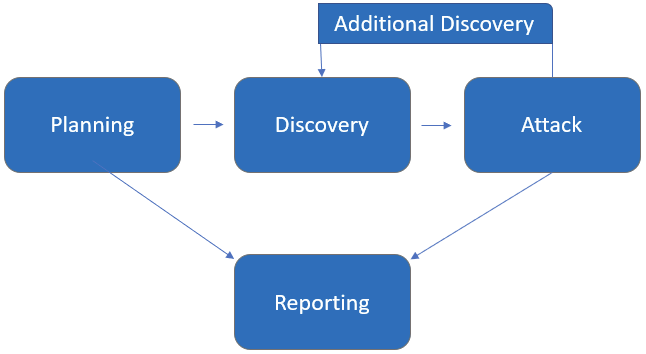
\includegraphics[width=\textwidth]{flow.png}
	\end{center}
	\pagebreak

	%%%%%%%%%%%%%%%%%%%%%%%%%%%
	%  Assessment Components  %
	%%%%%%%%%%%%%%%%%%%%%%%%%%%
	
	\boxsection{Assessment Components}
	
	\label{sec:assessment_components}
	A penetration test emulates the role of an attacker attempting to gain access to an internal network without internal resources or inside knowledge. \pentester attempts to gather sensitive information through open-source intelligence (OSINT), including employee information, historical breached passwords, and more that can be leveraged against external systems to gain internal network access. \pentester also performs scanning and enumeration to identify potential vulnerabilities in hopes of exploitation.
	

	%%%%%%%%%%%%%%%%%%%%%%%%%%%%%%%%%%%%%%
	%  Findings Severity Classification  %
	%%%%%%%%%%%%%%%%%%%%%%%%%%%%%%%%%%%%%%
	
	
	\boxsection{Findings Severity Classification}
	
	\label{sec:findings_severity_classification}
    
	The following table defines levels of severity and corresponding CVSS score range that are used throughout the document to assess vulnerability and risk impact.
	
	\begin{table}[htpb]
	    
	    \centering
	    \caption{Summary of the findings severity classification used.}
	    \label{tab:severityClassification}
	    \begin{tabular}{|p{2.5cm}|p{2.5cm}|p{9.5cm}|}
		\hline 
		\rowcolor{heading-grey}\multicolumn{1}{|>{\centering\arraybackslash}m{25mm}|}{\textcolor{white}{\textbf{Severity}}} & 
		\multicolumn{1}{>{\centering\arraybackslash}m{25mm}|}{\textcolor{white}{\textbf{CVSS v3 Score Range}}} & 
		\multicolumn{1}{>{\centering\arraybackslash}m{95mm}|}{\textcolor{white}{\textbf{Definition}}}  \\ \hline
		\cellcolor{Critical}\textcolor{white}{\textbf{Critical}} & 9.0-10.0 & Exploitation is straightforward and usually results in system-level compromise.  It is advised to form a plan of action and patch immediately. \\ \hline
		\cellcolor{High}\textcolor{white}{\textbf{High}} & 7.0-8.9 & Exploitation is more difficult but could cause elevated privileges and potentially a loss of data or downtime.  It is advised to form a plan of action and patch as soon as possible. \\ \hline
		\cellcolor{Medium}\textcolor{white}{\textbf{Medium}} & 4.0-6.9 & Vulnerabilities exist but are not exploitable or require extra steps such as social engineering.  It is advised to form a plan of action and patch after high-priority issues have been resolved.  \\ \hline
		\cellcolor{Low}\textcolor{white}{\textbf{Low}} & 0.1-3.9 & Vulnerabilities are non-exploitable but would reduce an organization’s attack surface.  It is advised to form a plan of action and patch during the next maintenance window.  \\ \hline \cellcolor{Info}\textcolor{white}{\textbf{Informational}} & N/A & No vulnerability exists.  Additional information is provided regarding items noticed during testing, strong controls, and additional documentation.  \\ \hline
	    
	    \end{tabular}
	    
	\end{table}


	%%%%%%%%%%%
	%  Scope  %
	%%%%%%%%%%%
	\newpage
	\boxsection{Scope}%
	\label{sec:scope}

    
	The overview of the scope of the engagement is described in Table \ref{tab:scopeEngagement}.
    

	\begin{table}[htpb]
	    
	    \centering
	    \caption{Scope of the engagement}
	    \label{tab:scopeEngagement}
	    \begin{tabular}{|p{5.5cm}|p{6.5cm}|}
	    \hline
	    \rowcolor{heading-grey}\textcolor{white}{\textbf{Description}} & \textcolor{white}{\textbf{IP Range}} \\ \hline
	    Web server & 10.10.10.0/24 \hfill\break random.com \\ \hline
	    \end{tabular}
	    
	\end{table}

	%%%%%%%%%%%%%%%%%%%%%%%%%%%
	%  Scope:Scope Exclusion  %
	%%%%%%%%%%%%%%%%%%%%%%%%%%%
	
	
	%\boxsubsection{Scope Exclusion}%
	%\label{sub:scope_exclusion}
	
	
	%Per client request, \pentesterShort\ did not perform any Denial of Service %attacks during testing.
	
	
	%%%%%%%%%%%%%%%%%%%%%%%%%%%%%
	%  Scope:Client Allowances  %
	%%%%%%%%%%%%%%%%%%%%%%%%%%%%%

	%\boxsubsection{Client Allowances}%
	%label{sub:client_allowances}
	
	
	%\companyNameShort\ did not provide any allowances to assist the testing.
	
	%\pagebreak
	
	%%%%%%%%%%%%%%%%%%%%%%%
	%  Executive Summary  %
	%%%%%%%%%%%%%%%%%%%%%%%
    \newpage
	\boxsection{Executive Summary}%
	\label{sec:executive_summary}
	
	
	PENTESTER evaluated \companyName' external security posture through an external network penetration test from December 2nd to December 9th, 2022. The test consisted of a series of attacks designed to uncover vulnerabilities in \companyName' systems. Unfortunately, \pentester found several critical vulnerabilities that could allow an attacker to gain full access to \companyName' internal network and control of the DMZ. It is highly recommended that \companyName address these vulnerabilities as soon as possible, as they are easily discovered and exploited with minimal effort. Failure to address these vulnerabilities could result in a significant security breach for \companyName.
	

	%%%%%%%%%%%%%%%%%%%%%%%%%%%%%%%%%%%%%%
	%  Executive Summary:Attack Summary  %
	%%%%%%%%%%%%%%%%%%%%%%%%%%%%%%%%%%%%%%
	
	\boxsubsection{Most Important Findings}%
	\label{sub:attack_summary}
	
	All findings, sorted by importance, are displayed in chapter 8 \hyperref[sec:vulnerabilitiesbyimpact]{Vulnerability by Impact}. The most important findings are:
	
	\begin{itemize}
	    \item 1
	    \item 2
	\end{itemize}
	
	\boxsubsection{Advice}%
	\label{sub:attack_summary}
	
	All findings in chapters 9 through 11 include steps on remediation. The most important remediation steps are:
	
	\begin{itemize}
	    \item 1
	    \item 2
	\end{itemize}
	
    %%%%%%%%%%%%%%%%%%%%%%%%%%%%%%%%%%%%%%
	%  Remediation report  %
	%%%%%%%%%%%%%%%%%%%%%%%%%%%%%%%%%%%%%%
	\newpage
	\boxsection{Remediation Report}%
	\label{sec:executive_summary}
    Lorem Ipsum is simply dummy text of the printing and typesetting industry. Lorem Ipsum has been the industry's standard dummy text ever since the 1500s, when an unknown printer took a galley of type and scrambled it to make a type specimen book. It has survived not only five centuries, but also the leap into electronic typesetting, remaining essentially unchanged. It was popularised in the 1960s with the release of Letraset sheets containing Lorem Ipsum passages, and more recently with desktop publishing software like Aldus PageMaker including versions of Lorem Ipsum.
	
	\boxsubsection{Remediation on Strategic Level}%
	\label{sub:attack_summary}
	
	Lorem Ipsum is simply dummy text of the printing and typesetting industry. Lorem Ipsum has been the industry's standard dummy text ever since the 1500s, when an unknown printer took a galley of type and scrambled it to make a type specimen book. It has survived not only five centuries, but also the leap into electronic typesetting, remaining essentially unchanged. It was popularised in the 1960s with the release of Letraset sheets containing Lorem Ipsum passages, and more recently with desktop publishing software like Aldus PageMaker including versions of Lorem Ipsum.
	
	\boxsubsection{Remediation on Tactical Level}%
	\label{sub:attack_summary}
	Lorem Ipsum is simply dummy text of the printing and typesetting industry. Lorem Ipsum has been the industry's standard dummy text ever since the 1500s, when an unknown printer took a galley of type and scrambled it to make a type specimen book. It has survived not only five centuries, but also the leap into electronic typesetting, remaining essentially unchanged. It was popularised in the 1960s with the release of Letraset sheets containing Lorem Ipsum passages, and more recently with desktop publishing software like Aldus PageMaker including versions of Lorem Ipsum.
    \\
    \begin{itemize}
        \item LOREM
        \item IPSUM
    \end{itemize}


    \boxsubsection{Remediation on Operational Level}%
	\label{sub:attack_summary}
	Lorem Ipsum is simply dummy text of the printing and typesetting industry. Lorem Ipsum has been the industry's standard dummy text ever since the 1500s, when an unknown printer took a galley of type and scrambled it to make a type specimen book. It has survived not only five centuries, but also the leap into electronic typesetting, remaining essentially unchanged. It was popularised in the 1960s with the release of Letraset sheets containing Lorem Ipsum passages, and more recently with desktop publishing software like Aldus PageMaker including versions of Lorem Ipsum.
    \\
    \begin{itemize}
    \item 1
    \item 2
    \item 3
    \item 4
    \end{itemize}
	
	%%%%%%%%%%%%%%%%%%%%%%%%%%%%%%%
	%  Vulnerabilities by Impact  %
	%%%%%%%%%%%%%%%%%%%%%%%%%%%%%%%

	\newpage	
	\boxsection{Vulnerabilities by Impact}%
	\label{sec:vulnerabilitiesbyimpact}
	    
        \begin{center}
	    \begin{tabular}{|l|p{0.85\textwidth}|l|p{0.8\textwidth}}
        \hline
        \rowcolor{dark-blue}
        \multicolumn{1}{|l|}{\textbf{\color{white}Impact}} & \textbf{\color{white}Finding} \\ \hline
        \cellcolor{Critical}\textbf{\color{white}Critical}    & \hyperref[critical:main]{Lorem ipsum}                \\ \hline
        \cellcolor{High}\textbf{\color{white}High}    & \hyperref[high:main]{Lorem ipsum}                \\ \hline
        \cellcolor{Medium}\textbf{\color{white}Medium}    & \hyperref[medium:main]{Lorem ipsum}                  \\ \hline
        \cellcolor{Low}\textbf{\color{white}Low}    & \hyperref[low:main]{Lorem ipsum}               \\ \hline
        \cellcolor{Info}\textbf{\color{white}Info}    & \hyperref[info:main]{Lorem ipsum}                \\ \hline
        \end{tabular}
        \end{center}
        
	
    

	%%%%%%%%%%%%%%%%%%%%%%%%%%%%%%%%%%%%%%%%
	%  Penetration Test Findings  %
	%%%%%%%%%%%%%%%%%%%%%%%%%%%%%%%%%%%%%%%%
	
	\newpage
	\boxsection{Penetration Test Findings - }[5 Findings]%
	\label{sec:external_penetration_test_findings}
	
	\textbf{The following findings have been written down in chronological order.}

	%%%%%%%%%%%%%%%%%%%%%%%%%%%%%%%%%%%%%%%%%%%%%
	%  Findings Subsections - Insert from HERE  %
	%%%%%%%%%%%%%%%%%%%%%%%%%%%%%%%%%%%%%%%%%%%%%
	
	    %%%%%%%%%%%%%%%%%%%%%%%%%%%%%%%%%%%%%%%%%%%%%
	%  Critical Finding                              %
	%%%%%%%%%%%%%%%%%%%%%%%%%%%%%%%%%%%%%%%%%%%%%

	\boxcriticalsection{Critical Finding (Critical 10.0)}[CWE 614]%
	\label{critical:main}
	\sethlcolor{criticalbox}
	
    Lorem Ipsum is simply dummy text of the printing and typesetting industry. Lorem Ipsum has been the industry's standard dummy text ever since the 1500s, when an unknown printer took a galley of type and scrambled it to make a type specimen book.
    
    \boxcriticalsectionsub{Impact}
    \label{critical:impact}
    Lorem Ipsum is simply dummy text of the printing and typesetting industry. Lorem Ipsum has been the industry's standard dummy text ever since the 1500s, when an unknown printer took a galley of type and scrambled it to make a type specimen book.

	\boxcriticalsectionsub{Method of Exploitation}%
	\label{critical:method_of_exploitation}
	
	%\begin{boxGrey}
	\begin{enumerate}
        \item 1.
        \item 2
        \item 3
    \end{enumerate}
    
    %configuring lstlisting
    \lstset{
            language=Python,
            basicstyle=\ttfamily\small,
            keywordstyle=\color{blue},
            stringstyle=\color{red},
            commentstyle=\color{green},
            backgroundcolor=\color{gray!15},
            lineskip={0.5},
            breaklines=true,
            breakatwhitespace=false,
            columns
        }

    \textbf{Some random python code}
    \begin{boxCode}
        \begin{lstlisting}
            import random

            def random_useless_code():
            x = random.randint(0, 100)
            y = random.randint(0, 100)
            z = x * y
            return z

            print(random_useless_code())

        \end{lstlisting}
    \end{boxCode}
    %\image[400pt]{image.png}{Description}

	%\end{boxGrey}

	\boxcriticalsectionsub{Remediation}%
	\label{critical:remediation}
	%\begin{boxGrey}
        \textbf{The following steps should be taken to remediate}
        	\begin{enumerate}
                \item 1.
                \item 2
                \item 3
            \end{enumerate}

	%\end{boxGrey}
	
	\boxcriticalsectionsub{References}
    \label{critical:references}
    %\begin{boxGrey}
    \begin{itemize}
    \item \url{https://clickeys.nl}
    \end{itemize}
    %\end{boxGrey}
	\pagebreak
	\newpage
	    %%%%%%%%%%%%%%%%%%%%%%%%%%%%%%%%%%%%%%%%%%%%%
	%  High Finding                              %
	%%%%%%%%%%%%%%%%%%%%%%%%%%%%%%%%%%%%%%%%%%%%%

	\boxhighsection{High Finding (High 8.0)}[CWE 614]%
	\label{high:main}
	\sethlcolor{highbox}
	
    Lorem Ipsum is simply dummy text of the printing and typesetting industry. Lorem Ipsum has been the industry's standard dummy text ever since the 1500s, when an unknown printer took a galley of type and scrambled it to make a type specimen book.
    
    \boxhighsectionsub{Impact}
    \label{high:impact}
    Lorem Ipsum is simply dummy text of the printing and typesetting industry. Lorem Ipsum has been the industry's standard dummy text ever since the 1500s, when an unknown printer took a galley of type and scrambled it to make a type specimen book.

	\boxhighsectionsub{Method of Exploitation}%
	\label{high:method_of_exploitation}
	
	%\begin{boxGrey}
	\begin{enumerate}
        \item 1.
        \item 2
        \item 3
    \end{enumerate}
    %\image[400pt]{image.png}{Description}

	%\end{boxGrey}

	\boxhighsectionsub{Remediation}%
	\label{high:remediation}
	%\begin{boxGrey}
        \textbf{The following steps should be taken to remediate}
        	\begin{enumerate}
                \item 1.
                \item 2
                \item 3
            \end{enumerate}

	%\end{boxGrey}
	
	\boxhighsectionsub{References}
    \label{high:references}
    %\begin{boxGrey}
    \begin{itemize}
    \item \url{https://clickeys.nl}
    \end{itemize}
    %\end{boxGrey}
	\pagebreak
	\newpage
	    %%%%%%%%%%%%%%%%%%%%%%%%%%%%%%%%%%%%%%%%%%%%%
	%  Medium Finding                              %
	%%%%%%%%%%%%%%%%%%%%%%%%%%%%%%%%%%%%%%%%%%%%%

	\boxmediumsection{Medium Finding (Medium 10.0)}[CWE 614]%
	\label{medium:main}
	\sethlcolor{mediumbox}
	
    Lorem Ipsum is simply dummy text of the printing and typesetting industry. Lorem Ipsum has been the industry's standard dummy text ever since the 1500s, when an unknown printer took a galley of type and scrambled it to make a type specimen book.
    
    \boxmediumsectionsub{Impact}
    \label{medium:impact}
    Lorem Ipsum is simply dummy text of the printing and typesetting industry. Lorem Ipsum has been the industry's standard dummy text ever since the 1500s, when an unknown printer took a galley of type and scrambled it to make a type specimen book.

	\boxmediumsectionsub{Method of Exploitation}%
	\label{medium:method_of_exploitation}
	
	%\begin{boxGrey}
	\begin{enumerate}
        \item 1.
        \item 2
        \item 3
    \end{enumerate}
    %\image[400pt]{image.png}{Description}

	%\end{boxGrey}

	\boxmediumsectionsub{Remediation}%
	\label{medium:remediation}
	%\begin{boxGrey}
        \textbf{The following steps should be taken to remediate}
        	\begin{enumerate}
                \item 1.
                \item 2
                \item 3
            \end{enumerate}

	%\end{boxGrey}
	
	\boxmediumsectionsub{References}
    \label{medium:references}
    %\begin{boxGrey}
    \begin{itemize}
    \item \url{https://clickeys.nl}
    \end{itemize}
    %\end{boxGrey}
	\pagebreak
	\newpage
	    %%%%%%%%%%%%%%%%%%%%%%%%%%%%%%%%%%%%%%%%%%%%%
	%  Low Finding                              %
	%%%%%%%%%%%%%%%%%%%%%%%%%%%%%%%%%%%%%%%%%%%%%

	\boxlowsection{Low Finding (Low 3.1)}[CWE 614]%
	\label{low:main}
	\sethlcolor{lowbox}
	
    Lorem Ipsum is simply dummy text of the printing and typesetting industry. Lorem Ipsum has been the industry's standard dummy text ever since the 1500s, when an unknown printer took a galley of type and scrambled it to make a type specimen book.
    
    \boxlowsectionsub{Impact}
    \label{low:impact}
    Lorem Ipsum is simply dummy text of the printing and typesetting industry. Lorem Ipsum has been the industry's standard dummy text ever since the 1500s, when an unknown printer took a galley of type and scrambled it to make a type specimen book.

	\boxlowsectionsub{Method of Exploitation}%
	\label{low:method_of_exploitation}
	
	%\begin{boxGrey}
	\begin{enumerate}
        \item 1.
        \item 2
        \item 3
    \end{enumerate}
    %\image[400pt]{image.png}{Description}

	%\end{boxGrey}

	\boxlowsectionsub{Remediation}%
	\label{low:remediation}
	%\begin{boxGrey}
        \textbf{The following steps should be taken to remediate}
        	\begin{enumerate}
                \item 1.
                \item 2
                \item 3
            \end{enumerate}

	%\end{boxGrey}
	
	\boxlowsectionsub{References}
    \label{low:references}
    %\begin{boxGrey}
    \begin{itemize}
    \item \url{https://clickeys.nl}
    \end{itemize}
    %\end{boxGrey}
	\pagebreak
	\newpage
	    %%%%%%%%%%%%%%%%%%%%%%%%%%%%%%%%%%%%%%%%%%%%%
	%  Info Finding                              %
	%%%%%%%%%%%%%%%%%%%%%%%%%%%%%%%%%%%%%%%%%%%%%

	\boxinfosection{Info Finding (Info 0.0)}[CWE 614]%
	\label{info:main}
	\sethlcolor{infobox}
	
    Lorem Ipsum is simply dummy text of the printing and typesetting industry. Lorem Ipsum has been the industry's standard dummy text ever since the 1500s, when an unknown printer took a galley of type and scrambled it to make a type specimen book.
    
    \boxinfosectionsub{Impact}
    \label{info:impact}
    Lorem Ipsum is simply dummy text of the printing and typesetting industry. Lorem Ipsum has been the industry's standard dummy text ever since the 1500s, when an unknown printer took a galley of type and scrambled it to make a type specimen book.

	\boxinfosectionsub{Method of Exploitation}%
	\label{info:method_of_exploitation}
	
	%\begin{boxGrey}
	\begin{enumerate}
        \item 1.
        \item 2
        \item 3
    \end{enumerate}
    %\image[400pt]{image.png}{Description}

	%\end{boxGrey}

	\boxinfosectionsub{Remediation}%
	\label{info:remediation}
	%\begin{boxGrey}
        \textbf{The following steps should be taken to remediate}
        	\begin{enumerate}
                \item 1.
                \item 2
                \item 3
            \end{enumerate}

	%\end{boxGrey}
	
	\boxinfosectionsub{References}
    \label{info:references}
    %\begin{boxGrey}
    \begin{itemize}
    \item \url{https://clickeys.nl}
    \end{itemize}
    %\end{boxGrey}
	\pagebreak
	    
	%%%%%%%%%%%%%%%%%%%%%%%%%%%%%%%%%%%
	%  Additional Reports and Scans   %
	%%%%%%%%%%%%%%%%%%%%%%%%%%%%%%%%%%%

	\newpage
	\boxsection{Summary of Exploited Machines}%
	\label{summary}
	
        \begin{center}
	    \begin{tabular}{|p{2.5cm}|p{2.5cm}|p{2.5cm}|p{2.5cm}|p{2.5cm}|}
	    \hline
	    \rowcolor{heading-grey}\textcolor{white}{\textbf{Host}} & \textcolor{white}{\textbf{Open Ports}} & \textcolor{white}{\textbf{Services}} & \textcolor{white}{\textbf{Access}} & \textcolor{white}{\textbf{Exploited}} \\ \hline
	    lorem & lorem & lorem & lorem & lorem \\ \hline
        lorem & lorem & lorem & lorem & lorem \\ \hline
        lorem & lorem & lorem & lorem & lorem \\ \hline
        lorem & lorem & lorem & lorem & lorem \\ \hline
        lorem & lorem & lorem & lorem & lorem \\ \hline
        lorem & lorem & lorem & lorem & lorem \\ \hline
	    \end{tabular}

        \end{center}

\end{document}


